% Main document PNSAC newsletter
% Language: Latex
%

% ................................................................... %
% Preamble .......................................................... %

\documentclass[a4paper]{report}


% Use named colours (68 standard colours known to dvips)
\usepackage[usenames,dvipsnames]{color}
\usepackage{yfonts,color}

\usepackage{amssymb,amsmath}

% Note: Need to include amsmath before PNSAC, because the latter redefines the
% equation environment.
\usepackage{../PNSAC} 
\usepackage[round]{natbib}
% To control float placement
\usepackage{stfloats}
\usepackage{float}

% for Sweave
\usepackage{listings}

% for tcltk-update
\usepackage{shortvrb}

%\usepackage{chapterbib}
\sloppy{}

% Use rotating package to typeset images in landscape mode
\usepackage{rotating}

% Using caption package and \caption* to exclude figure numbers.
\usepackage{caption}

% Using subfigure package (for side-by-side images).
\usepackage{subfigure}

% Using package for Initial drop capitals
\usepackage{lettrine}

% ................................................................... %
% Begin document .................................................... %

\begin{document}

\volume{16} % \volnumber{1}
\issue{2}
\date{September 2020} 
\titlepage

%\centerline {\Large \textit {Celebrating the 70th Anniversary of the First
%Canadian Non-Stop Transcontinental Flight}}

% Editor's notes
% ..................................................... %

% Editor's notes
\begin{article}
	% Template PNSAC newsletter - Article % Language: Latex
%

% Head



\title{Editor's Notes} 
\author{Roger Button}

\maketitle


\end{multicols}


\vspace{12pt}

Putting out this edition of the Chronicle has been an example of great
co-operation from members and non-members alike. Thanks are owed to a
number of people. Our member Gary Whitten was instrumental in getting
the necessary permission from Air Force Magazine to publish the
"Diversion to Alert" article.  

%Allan Bowes, another member, suggested
%that we should try to get the "Civil Merlins" article into an edition
%of the Chronicle.  Following his suggestion we contacted Ben Dunnell,
%the editor of Aeroplane Magazine. Through Ben's offices we were able to
%secure permission to reprint this article.  The "Civil Merlins" was
%part of a comprehensive 17 page Aeroplane Database article on the
%Merlin. If any members wish to read the entire article it was published
%in the July 2017 issue.

In addition thanks go out to the other contributors, namely Richard
Lodge, Garry Dupont,  Neil Raynor, and R\'{e}jean Demers. A special thanks
to Bruce Gemmill who took the lead in putting together the progress report,
which can be found in the Conservator's Corner section.

Finally, I would like to thank Drew Hodge our stalwart publisher of this
edition. We do appreciate receiving feedback from our readers including
comments on the articles or suggestions for new articles. We are always on the
lookout for content for the Chronicle so please do not hesitate to bring
forward any ideas that you might have. As noted in the Conservator's Corner
article the restoration of engine number 4 has been completed. Our next
edition will focus on the engine restoration work so if you have any material
or comments specific to that aspect of the restoration please let us know.
Enjoy.


\vspace{12pt}


\begin{footnotesize} \raggedleft PNSAC\\
\end{footnotesize}

\begin{multicols}{2}

% End of text.

%%% Local Variables: %%% mode: latex %%% TeX-master: main_document.tex
%%% End:
 
\end{article}

\pagebreak

% President's report
%................................................. %

% Report
\begin{article}
	% Template PNSAC newsletter - Article
% Language: Latex
%

% Head

\title{Notes from the President}
\author{Richard Lodge}

\maketitle

As I write these notes in the middle of April, I see a fresh fall of
snow on the ground.  For the first time in many years, the North Star,
already out in the open, will be covered in snow.  This unusual
situation has been caused by the Star Wars exhibition to be located in
the Storage Hangar this summer.  The larger Argus airplane has also
been moved outside, in a position which reduces visibility of the
North Star for the public.  This will present a challenge to us in
showing off our work to Museum visitors.

The Star Wars exhibition has also affected our plans for commemorating
the 10th anniversary of the founding of the Project North Star
Association.  We are now planning to celebrate the anniversary when we
open the North Star for the public on Canada Day.  That will be the
only time this summer when we can invite the general public to see the
North Star and offer our members conducted tours inside the plane.  We
will ensure that there are good directions to the North Star and
volunteers located in the main Museum will assist visitors and members
in finding it.

All this has had only a minor effect on the plane restoration.  We are
very actively working both inside the restoration shop and inside the
plane itself.  As usual our Project Manager has provided elsewhere in
the Chronicle a comprehensive report of our progress.

In the next Chronicle, we are planning to start a Letters to the
Editor section.  Many of our members are not located in Ottawa and may
well have interesting questions or comments on our work, or stories or
pictures about North Star in general.  We will welcome any letters or
stories, which should be sent to the Editor
(\email{editor@projectnorthstar.ca}) by email or by mail to the
address shown on the last page of this newsletter.  As with any
publication, our editor will decide whether an item should be
published.


\begin{footnotesize}
    \raggedleft PNSAC\\
\end{footnotesize}

% End of text.

%%% Local Variables: 
%%% mode: latex
%%% TeX-master: main_document.tex
%%% End: 

 
\end{article}

\pagebreak

% Special
\begin{article}
	% Template PNSAC newsletter - Article
% Language: Latex
%

% Head

\title{PNSAC Merchandise}
%% \author{Drew Hodge}

\maketitle

%\end{multicols}

\begin{figure}[ht!]
   \vspace{2em}
   \centering
   %name of the graphic, without the path AND in EPS format:
   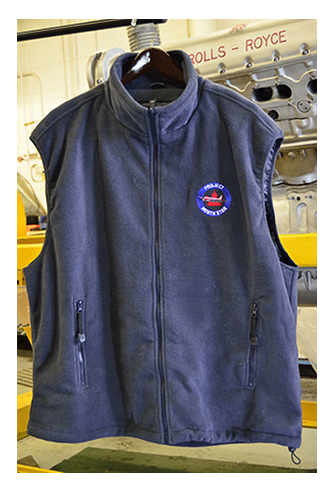
\includegraphics[scale=1.0]{fleece_YOW7578.eps}
   %caption of the figure 
   \caption*{\small \em PNSAC winter apparel}
   %label of the figure, which has to correspond to \ref{}:
   \label{fig:merchandise}
\end{figure}



The first frost warnings on the Weather Channel are reminders that
fall and winter are just around the corner. Keep warm on those frosty
fall days with a PNSAC toque and sweatshirt. We can also take
individual orders for the micro fleece vests shown in the photo on the
left, and if you're looking for early Christmas presents, how about a
coffee mug or a t-shirt?

See our Facebook page,
{\normalfont\color{blue}\texttt{\href{https://www.facebook.com/media/set/?set=a.610706705637878.1073741851.284829008225651&type=1}{PNSAC
      Merchandise}}}, for details about what we're offering, and place your
orders by sending an email message to the following address
\email{pnsac.merchandise@gmail.com}.

For members in the Ottawa-Gatineau region, you can arrange to pick up
your merchandise at the Canada Aviation and Space Museum any Monday or
Tuesday, between 10:00 AM and 3:00 PM. We can also ship your purchases
to you for an extra fee. Please specify museum pickup or shipping with
your order.

Merchandise is also available during our Quarterly Meetings
at CASM.

Look forward to hearing from you.

``The Merchandise Committee''

 



\begin{footnotesize}
    \raggedleft PNSAC\\
\end{footnotesize}

%\begin{multicols}{2}

% End of text.

%%% Local Variables: 
%%% mode: latex
%%% TeX-master: main_document.tex
%%% End: 

 
\end{article}

%\pagebreak

% Progress report ................................................... %

% Report
\begin{article}
	
% Template PNSAC newsletter - Article
% Language: Latex
%

% Head

\title{Project Manager's Progress Report}
\subtitle{April 2013}
\author{Bruce Gemmill}

\maketitle

During the last three months we have continued working on our two top
priorities -- Engine \#3 and the interior of the North Star.  Some of
the external skin has also been polished.  Volunteers were also
involved in preparing the North Star and Argus for an early move
outside, to accommodate an exhibit in the Storage Wing.

\section{Engine and QEC}
\label{sec:engines}

The engine rebuild is nearing completion, with magnetos and a few
other accessories to be installed.  The completed engine will soon be
installed in the engine frame, then work will begin on the
supercharger and intercooler.

\begin{figure}[htbp]
   \vspace{2em}
   \centering
   %name of the graphic, without the path AND in EPS format:
   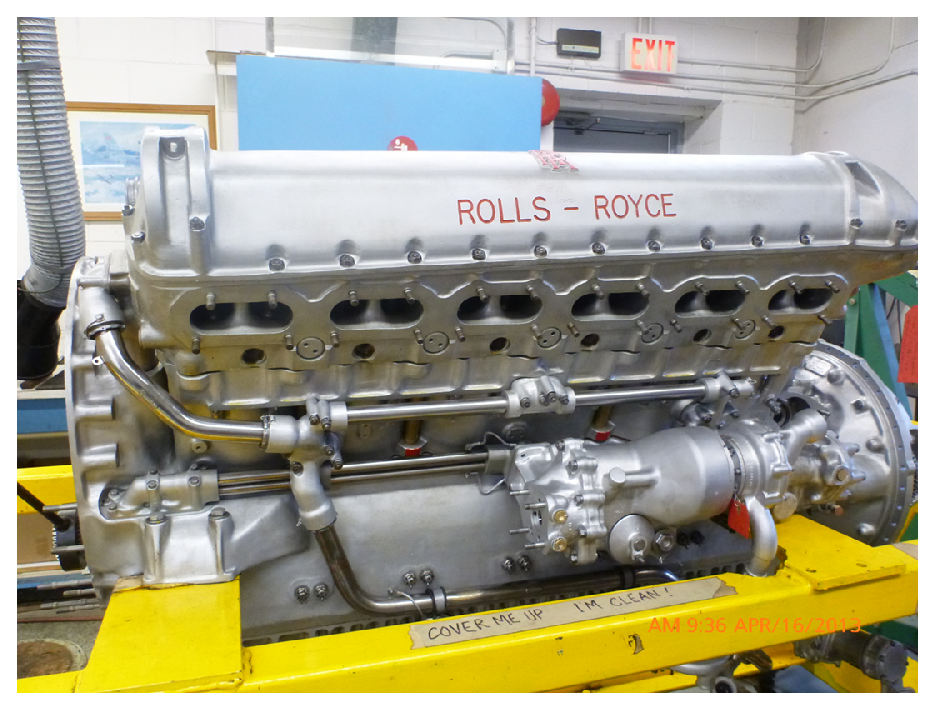
\includegraphics[scale=0.5]{engine3.eps}
   %caption of the figure 
   \caption*{\small \em North Star engine 3.}
   %label of the figure, which has to correspond to \ref{}:
   \label{fig:engine3}
\end{figure}


The basic engine frame is back together.  The three radiator sections
were cleaned and painted, then attached to the front of the frame.
The rear cowl ring has been disassembled, and new mounting hardware is
being fitted before the parts are painted and reassembled.  The front
cowl assembly (radiator cover) has also been cleaned, repaired and
polished, ready to install.  Other cowl panels will each be cleaned,
repaired and polished, ready to install once the complete engine is in
place.  Work is also underway on a host of pipes, cables, accessories
and fittings needed to complete the assembly of the engine and QEC
prior to installation on the aircraft.

As mentioned, volunteers worked to prepare the North Star for an early
move outside.  Besides installing windows and closing other openings
for weather protection, propeller \#2 was installed on engine \#2,
rather than keeping it stored in the hangar.

\section{Fuselage and Crew Area}
\label{empennage}

The crew lounge and forward washroom are looking more finished,
although much work still remains.  New Plexiglas windows were
installed in the crew lounge, washroom and APU closet.  The water tank
was installed in the ceiling, and the water lines hooked to the newly
refurbished sink. 
 
The air scoop that supplied cold air to the Janitrol heaters was badly
corroded and removed for repair.  This involved cutting away damaged
aluminum and riveting carefully formed patches in place.  The assembly
was primed, then riveted back in place over the crew lounge.  New
insulation was installed in the ceiling, including a layer of heat
resistant mica.  Some pipes and wires have been installed, and the
heating ducts were cleaned and recovered with fabric.  These will be
installed once the Janitrol heaters are in place.

The new galley is almost complete.  After the original doors are
repaired they will be attached to the new assembly, which can then be
installed in the crew lounge, just behind the equipment rack.  New
wiring legends were produced for the inside of the electrical
cabinets.  These will be laminated before installation, to prevent
deterioration from humidity.

The ceiling and wall panels in the forward and rear belly compartments
have been stencilled and installed.  The floor panels were badly
scratched and in some cases stretched, due to the heavy load of
baggage often carried in these compartments.  Each panel is being
assessed, and several have already been remade.  These will be painted
and stencilled, then installed later this spring.

One of the new de-icing boots has been successfully manufactured.
This will be an on-going project, as time permits.  Completed boots
will be stored until other repair work on wings and stabilizers has
been completed.

Work has begun manufacturing a full set of troop seats for the
aircraft.  A total of 33 seats will be sewn and fitted to new mounting
frames.  A design has been completed and fabric work has started.
Some of the fittings have also been made.  This work will continue for
some time and all completed items will be stored until the main cabin
has been repainted. 


\begin{figure}[htbp]
   \vspace{2em}
   \centering
   %name of the graphic, without the path AND in EPS format:
   \includegraphics[scale=0.5]{sink_vanity.eps}
   %caption of the figure 
   \caption*{\small \em Forward vanity.}
   %label of the figure, which has to correspond to \ref{}:
   \label{fig:vanity}
\end{figure}

The forward washroom has most equipment returned, including the toilet
and the window, minus the Plexiglas insert that is on order.
Likewise, the vanity mirror and various fixtures were repainted and
re-installed.  The door will not be installed until the new flooring
is glued down, one of the last tasks in the crew area.

The APU compartment, which had been converted to luggage and coat
storage, has been re-assembled.  The power inverter and cabinet were
re-installed, along with the luggage shelf and floor.

% The heater and ducting has become a major item of work.  All the ducts
% were removed and cleaned, but new woven fibreglass coverings will need
% to be attached.  Material is on order.  The main air scoop that feeds
% the heater was removed and found to be badly corroded.  This item is
% being rebuilt and must be installed before the aircraft goes outside
% this spring.

% Work also continues on the floor, ceiling and wall panels from the
% under floor belly compartment.  Some damaged panels may need to be
% replaced.  Progress is also being made on the de-icing boots for the
% wings

% We made good progress on our plan to build a set of troop seats for
% the aircraft.  Our appeal for donations was highly successful, and
% most of the material needed for the seats has now been received.
% Numerous fittings were manufactured and painted, and are stored until
% the seats are ready to install. 

\section{Planned Restoration Work--2013}
\label{sec:plannedwork}

This summer we will replace all the items removed from the crew areas
and continue the rebuild of engine \#3.

Sewing of the seat fabric will begin soon and will continue until all
the fabric has been stitched together.  The frames will be
manufactured later this year

Next we expect to begin work to restore the main cabin.  This will
require removal of the wood cargo floor for a thorough cleaning and
inspection.  We expect to find some corrosion damage that will require
repair. 


%% \begin{figure}[htbp]
%%    \vspace{2em}
%%    \centering
%%    %name of the graphic, without the path AND in EPS format:
%%    \includegraphics[scale=0.5]{MerlinCylinderHead.eps}
%%    %caption of the figure 
%%    \caption*{Richard Lodge and Garry Dupont, Merlin Cylinder Head}
%%    %label of the figure, which has to correspond to \ref{}:
%%    \label{fig:eng_one}
%% \end{figure}

\begin{footnotesize}
  \raggedleft PNSAC\\
\end{footnotesize}

% End of text.

%%% Local Variables: 
%%% mode: latex
%%% TeX-master: main_document.tex
%%% End: 

 
\end{article}

\pagebreak

% Member interview ................................................... %

% Report
\begin{article}
    % Template PNSAC newsletter - Article
% Language: Latex
%

% Head

\title{Our Members}
\author{This is the edited transcript of an interview with Garry Dupont by Richard Lodge.}

\maketitle

\textit{Garry why did you join Project North Star?}

I joined it when I was working full time and it was a discussion between me and
my wife as I knew retirement was looming and it was what I was going to do. I
had seen the article that was in the Ottawa Citizen with Robert Holmgren and Tim
Timmins requesting people to attend a meeting starting the project, and my wife
suggested I go to it, which I did and it gave me something to look forward to.
Even when I was employed I was able to physically contribute by coming in the
odd day and helping out with special projects and overhaul a few components and
stuff like that.\\

\noindent\textit{So you worked only in the engine shop?}

No.  When initially I was working, I worked on various other things and only
after I fully retired, I showed up and said Mike Irvin "I am here. I'll be here
for four days a week".  That's when he asked me to go into the engine shop
because they needed help in there.\\

\noindent\textit{Could you have worked anywhere but you chose to work in the engine shop?}

Actually, Mike chose for me.  Mike was the one who said go to the engine shop.\\

\noindent\textit{When you started with Project North Star would you have felt
that you had most experience of aviation work on engines, or could you gone
anywhere on the plane?}

I could have gone anywhere on the plane. Of this particular engine I had no
knowledge. I had never worked on these liquid cooled engines before.  I never
worked on a piston engine of that size before and actually I hadn't worked on
piston engines for quite a number of years because with my employment most of my
airplanes were with turbines.  We had some small piston engined airplanes of
which I had limited experience.\\

\noindent\textit{So quite a bit of your work in the engine shop was a learning
experience apart from learning about how the Merlin 622 was assembled, you were
also learning a bit about actually working on a large piston engine aircraft?}

That's correct and the systems on this particular engine were completely
different from anything I had ever worked on and I came across  an RCAF training
manual, which somebody had donated and I took it home and read it from one end
to the other over a couple of weeks. I was able to learn a considerable amount
about the engine and understand the systems and it started making sense to me,
so when you start assembling and disassembling and you look at a line you know
what that the line is for. You know what the electrical connections are for. You
know what system they belong to so it makes that part of the process much
easier.\\

\noindent\textit{I know from when we first started working together, you said
you worked for Perimeter Airlines in Winnipeg.  When you were working for
Perimeter, you were working mostly on Metroliners. Correct?}

Yes.  We had 2 Metroliners when I was there, but we also had 4 piston operated
Beechcraft Queenairs, we had 6 other Beechcraft.\\

\noindent\textit{When you worked at Perimeter, were you working on any part of
the plane and you weren't specialising in any particular part, so moving into
solely engines was really a new area of work for you?}

That's correct.\\

\noindent\textit{When you first started working in the engine shop, who were you
working with?}

There was Ted Devey, John Tasseron, Michel Lacasse and two other
fellows, the names escape me.\\

\noindent\textit{I asked a few minutes ago.  If you were only interested in
working on the engines.  Where else would you like to work on the plane? So you worked only in the engine shop?}

Anything actually, I don't do well with sheet metal work, I have done some,
minor bits. I could develop those skills a bit better.  Hydraulic systems; I
have a fairly good interest in, landing gear, the flaps, the hydraulics and all
those systems.  I have learned where the pumps are and how all that works now.
I have also read up little bit on the landing gear to understand it a bit better
and how it works and that would be interesting.\\

\noindent\textit{So you could, if they had been doing the landing gear at the
time you started have been quite interested in working on that side of things?}

Yes.\\

\noindent\textit{What would you say in retrospect was the most difficult part of
the work you were having to do on engines 3 and 4?  Was it lack of paperwork,
was it corrosion or what was it?}

The most difficult part was dealing with corrosion because of the amount of
corrosion in the engine and also the decision-making between my career and what
I would do and what the museum wanted in restoration. The hardest learning part
was learning about restoration and how to do it properly. I have had some good
mentors.  and I have learned fairly well on what is required to do and what to
look forward to in the future when planning the project; how to tackle it from a
restoration perspective rather than a maintenance perspective.\\

\noindent\textit{Was Mike Irvin one of your mentors helping you to know the
various procedures needed for restoration?}

Yes, Mike was the main mentor.  He was the one that took me under his wing and
showed me the requirements and the basis of doing restoration.\\

\noindent\textit{When you started working there, you weren't really in charge of
the engine because it was a combination of you and Ted Devey who was still
working there and who had worked on engines 1 and 2.  So you were working with
him under Mike Irvin?}

Yes.  That's right.\\

\noindent\textit{You feel one of the most difficult parts was to make the shift
from keeping an aircraft flying to restoring and conserving everything?}

That's right, yes.\\

\noindent\textit{Having done that and got into that sort of mindset, what would
you feel was the most difficult part of doing the engine, of restoring the
engines that you had to be involved with, or you had to work with.  Which part,
I am thinking of?}

The biggest part with the engines was the cleaning.  Believe it or not, the
engines and the old oil had been sitting there for 35 years, it was very
congealed and very difficult to remove.  Cleaning with solvents is not a
pleasant thing to do and that was about the only method we could use was to
clean and put it in the parts washer.  Once you put a part in the parts washer
you also had to be very careful because if it was steel, when it was removed
from the part washer it would flash freeze almost immediately, so it had to be
removed and treated straightaway with some sort of preserving oil to prevent the
surface from oxidizing.\\

\noindent\textit{I very much remember John Tasseron working on the pistons and
all work of getting the pistons out of the block  and then John working on the
cleaning the piston rings.  Were you very much involved in that side of things?}

Yes.  Cleaning up the piston rings was a real tedious job where you could spend
a whole week on one piston ring trying to free it up by scraping away the
corrosion, by tapping it to free the rings.  Sadly, a lot of them broke.  There
was nothing we could do to free them up.  We tried various chemicals, soaking
procedures, vibration procedures, putting them in sonic cleaners so that the
vibration would free up the dirt, but nothing seemed to work really well, except
getting in there with a little scraper and trying to scrape them clean.\\

\noindent\textit{And when you did manage to free the parts and get them clean,
you couldn't use a glass bead machine to do any cleaning because the parts were
aluminum so we had to use Scotch Brite and other things to clean them?}

Correct.  The purpose of glass beading is to remove corrosion and not to clean.
If you glass bead a surface, it changes the outer texture of it considerably. In
the engine shop we had at Perimeter, the only time they used glass beading was
for removing the outside surface of the engine block and then they could prepare
it for painting.\\

\noindent\textit{Now that you have finished the main part of the work on engines
3 and 4, what are the main additional parts or work still to be done on engines
3 and 4 and maybe on engines 1 and 2?}

R\'{e}j [Demers] wants to remove the engines so we will reinstall engine 4 when
it is ready and then we will go back and will work on each engine successively
and then work on the firewall and behind the firewall with the engine removed.
At the time when we do this we will inspect the engines to see if corrosion has
come back in some areas and I notice on some of the engines during Canada Day
when we removed parts and cowlings to display the engine that there was
corrosion showing up in certain areas where it had not been treated properly.
So when we remove the engines, and R\'{e}j agrees with me, we will put them back
in the engine shop and go over them thoroughly.  We have also found some issues
with some of the cowl parts just not being adjusted properly.  So in the end, I
would like to have all four engines installed on the wings properly treated so
that we don't have to worry about them again and also the cowls adjusted and
done properly so that at any time we can remove the cowl parts and reinstall
them with ease.  So that in the future, if you want to display the engine again,
you could effectively remove all the cowls on all four engines with ease and
then reinstall them without making any big issue of it.\\

\noindent\textit{Effectively you have got to remove any distortions in the cowl
panels. So those are the things to be done?  When you are finished working on
the Merlin engines, what would you like to do?  This is purely a personal thing
and nothing to do with the Museum.  More engines on a different plane or working
on the airframe?}

It really doesn't matter to me, whatever the Museum sees fit as a project, I am
willing to tackle it. 


% \end{multicols}

%\begin{quotation}
%	\textit{Jim Riddoch is one of the earliest and longest serving members of the
%Association. He has made a significant contribution to the operations of the
%Association including working on the aircraft as well as being an officer and
%member of the board of directors. Although officially retired from formal
%positions in the organization, he can still be counted on to help out when
%needed.}
%\end{quotation}

% \begin{multicols}{2}





%1.\textit{What is your background in aviation?}
%
%
%2. \textit{How long have you been involved with Project North Star and how and
%why did you get involved?}
%
%3. \textit{What has been the history of your involvement to date?}
%
%4. \textit{What has been the highlight of your involvement?}
%
%5. \textit{What has been the most challenging part of your involvement?}

\begin{footnotesize}
    \raggedleft PNSAC\\
\end{footnotesize}



% End of text.

%%% Local Variables: 
%%% mode: latex
%%% TeX-master: main_document.tex
%%% End: 

 
\end{article}

%\pagebreak

% Features
% ........................................................... %

% Feature article

\begin{article}
	% Template PNSAC newsletter - Article
% Language: Latex
%

% Head

\title{My Days at the Home of the Merlin Engine}
\author{Richard Lodge}

\maketitle

I am a bean counter and I always wanted to be an engineer. For 5 plus
years in the late 1950s I had struggled to overcome the boredom of
training to be a Chartered Accountant in Leeds in Northern England. We
worked long hours for free because it was said that our bosses would
be giving us a valuable training.

\end{multicols}

\begin{figure*}[ht!]
   \vspace{2em}
   \centering
   %name of the graphic, without the path AND in EPS format:
   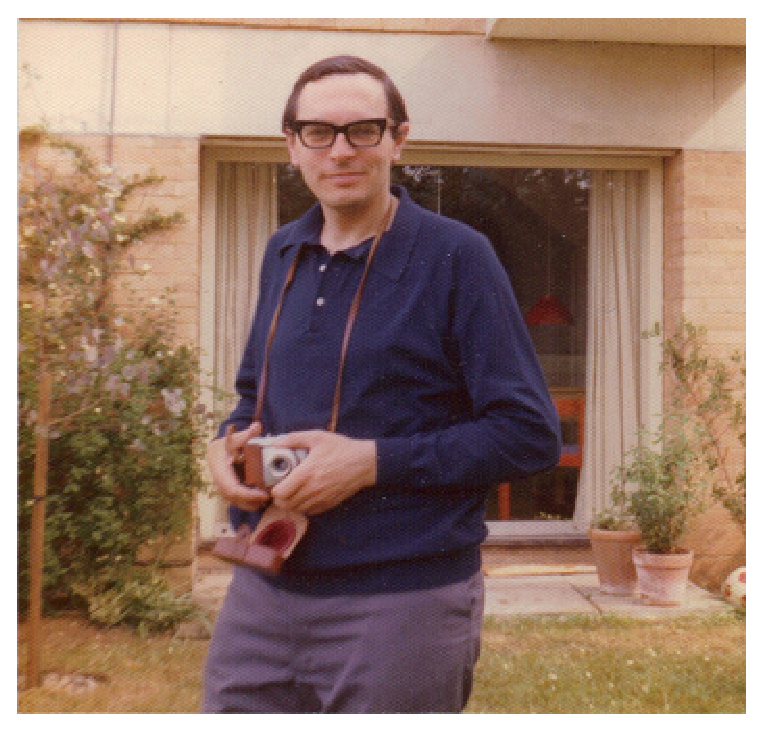
\includegraphics[scale=1.0]{richard_lodge.eps}
   %caption of the figure 
   \caption*{\small \em Richard Lodge in the 1970s.}
   %label of the figure, which has to correspond to \ref{}:
   \label{fig:richard}
\end{figure*}

\begin{multicols}{2}

Most of my friends were at university and enjoyed long summer holidays
when they would spend time tinkering with unreliable prewar old cars
while I toiled away in an office. Weekends were supposed to be spent
studying for accountancy exams. I always did the minimum amount of
study and would move into my father's big old garage at the earliest
opportunity to tinker with my 1934 Daimler limousine. The most common
tools I had to use were my hands, Whitworth spanners, feeler gauges, a
good sized hammer and Swarfega for cleaning up before doing a little
lightweight courting in the evenings.

Eventually the prized certificate arrived in the mail saying that I
had qualified as a Chartered Accountant. I was now ready to leave the
accountants' office behind and get a job as an accountant in
industry. I could hardly believe my luck when I was offered a job as
an assistant accountant in the Aero Engine Division of Rolls-Royce in
Derby.

\end{multicols}

\begin{figure*}[ht!]
   \vspace{2em}
   \centering
   %name of the graphic, without the path AND in EPS format:
   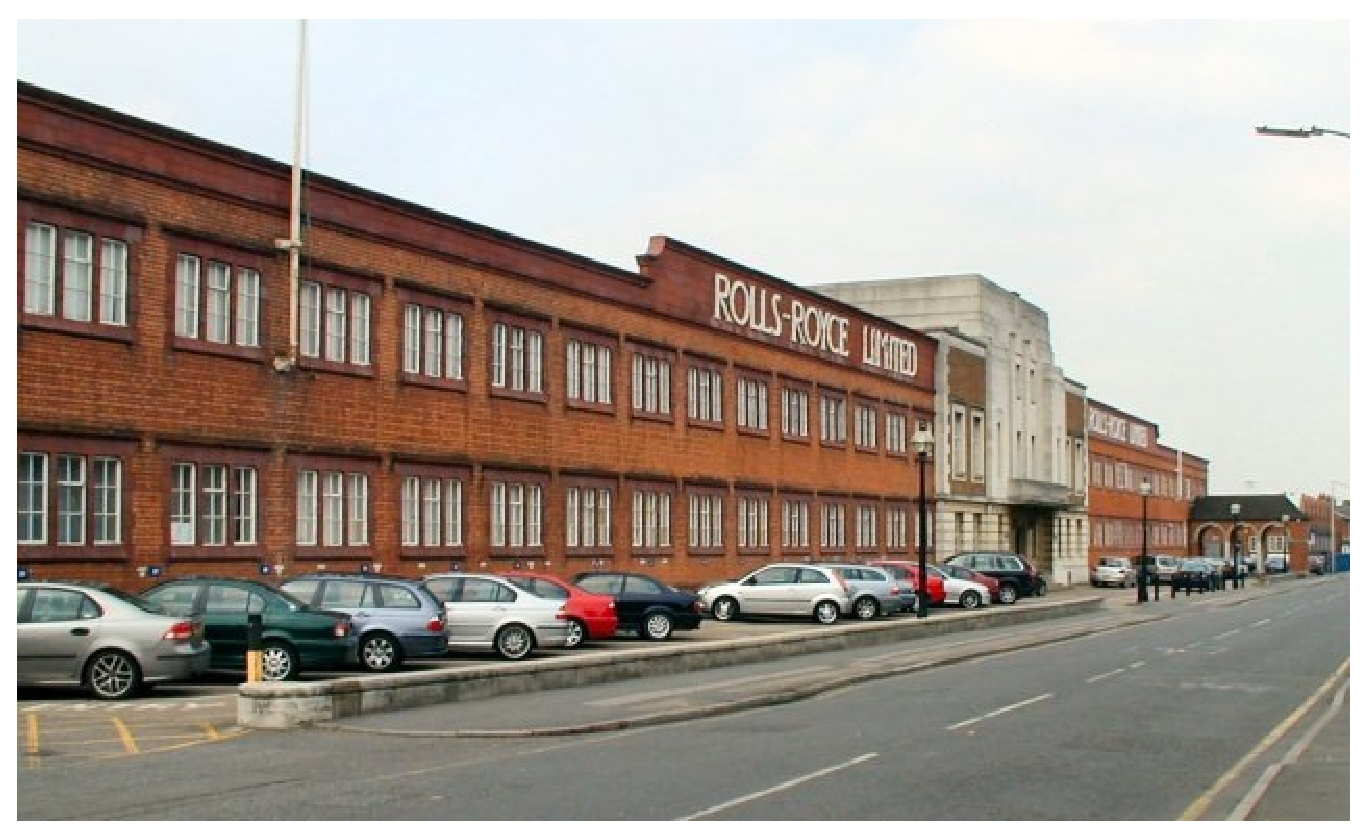
\includegraphics[scale=0.75]{rolls_royce.eps}
   %caption of the figure 
   \caption*{\small \em Nightingale Road office before closure in 2008.}
   %label of the figure, which has to correspond to \ref{}:
   \label{fig:rollsroyce}
\end{figure*}

\begin{multicols}{2}

As a young accountant I was very proud of myself to have got a job
with such a prestigious company and I duly reported to work on my
first Monday to be told that I would be given an induction period
under the guidance of an experienced employee. I found I was put with
two other green accountants to be guided by a man who was an ex WW2
regular army sergeant. He was about a foot shorter than me with a
pencil moustache but had a typical sergeant's voice and manner. Les
Hart knew very little about accounting and almost nothing about
engineering but he certainly knew the company and the world. One of
the best bits of advice he gave me was ``Do not let the buggers get you
down''. I needed this advice on many occasions while at Rolls-Royce.

Following a bewildering first week of being shown round some of the
R-R factories in Derby with my fellow new accountants, Les said we
were ready to start work. I was told to report to the Overheads
Department in the main accounting building near the Nightingale Road
head office. Les introduced me to the supervisor of the department and
then went on his way to deal with some other task. At that time R-R
employed about 30,000 people in several factories around the UK and I
felt very far removed from actual aero engines while sitting in this
vast sea of clerical people. The building was a converted warehouse
and my office was in the middle of the huge second floor housing about
200 people. There was no air conditioning and very little
ventilation. As the day wore on the atmosphere became putrid to say
the least of it. My pleasure at being offered a job at Rolls-Royce was
rapidly evaporating.

Derby in the 1960s was a two industry town, Rolls-Royce and the main
railway workshops of the Midland Region of British Railways. For many
people there were few choices other than to work at one of these two
employers. Many of the employees at R-R had been with the company
since leaving school at 16. They really did not like young
inexperienced accountants being foisted upon them but I was new, full
of enthusiasm and did not realize this.

The old sweats in the Overheads Department soon let me know that I
might be more technically qualified than them but that was only an
illusion. After a month or two, I made a bad mistake and my section
leader came to me and said ``You made a bad drop-off there''. I had no
idea what a drop-off was. He then called over the supervisor to
discuss the mistake and said ``Lodge here doesn't know what a drop-off
is and I guess he doesn't know whether he is punched, bored or
countersunk either.'' By that time I knew exactly what my mistake was
but what neither of these men explained was the meaning of their other
comments. It took me some time to find Les Hart who told me that a
drop-off referred to a careless person in the factory allowing an
expensive part to drop onto the floor and break and secondly that
punched, bored or countersunk described the method of making a certain
part of my anatomy. I was beginning to realize that to survive at R-R
I had a lot to learn.

Shortly afterwards I got my own back on these gentlemen when, to their
horror, I was appointed supervisor of the Overheads department.

In the next article I will describe how I came to enjoy the rest of my
time at R-R and learnt about life in the real world of traditional
British engineering.

\begin{footnotesize}
    \raggedleft PNSAC\\
\end{footnotesize}

% End of text.

%%% Local Variables: 
%%% mode: latex
%%% TeX-master: main_document.tex
%%% End: 

 
\end{article}

\pagebreak

% Feature article
\begin{article}                 
	% Template PNSAC newsletter - Article
% Language: Latex
%

% Head

\title{RAPCAN visits CASM}
\subtitle{Retired Airline Pilots of Canada Visit the Canada Aviation and
  Space Museum}
\author{Bill Tate}

\maketitle

At a monthly luncheon meeting of Retired Airline Pilots of Canada,
Captain Jim Strang, retired A-340 Captain, advised me the annual
general meeting for RAPCAN would be held in Ottawa in September
2012. Jim asked me if Project North Star Association of Canada could
assist the Ottawa Chapter of RAPCAN in making sure all would have a
good time.

Our guests would want to visit the North Star, and they would also
like to see the DC-9 and the F-86 in the storage hangar. Many of them
started their early jet experience flying the Sabres and had their
command promotion on the DC-9. These visits were quickly approved,
along with the booking of the Bush Theatre with the assistance of
Stephen Quick, Director General of the CASM.

RAPCAN had no idea how many people would be coming to Ottawa. Based on
previous annual general meeting attendance, from a low of 30 to a high
of 300, a figure of 125 was suggested for planning purposes. Next
question, how many people would want to come to the CASM and see the
North Star versus the Vintage Wings of Canada Air Show?

As we got closer to the date, the North Star visit was chosen by 71
visitors and 75 attended the Air Show. Our own Mike Irvin made sure
that the DC-9 was shown in the best possible way, and PNSAC volunteers
assisted through the day. Among our guests there were several former
North Star pilots for Trans Canada Airlines who added interesting
insights into that aircraft.

Ron Lemieux, former Director of Protocol at Rideau Hall, was
instrumental in ensuring a private tour of the Governor General's
Residence . All members of that tour were impressed with the history
and beauty, and with the kindness of staff who assisted those with
mobility issues.

The day started with Richard Lodge welcoming the group in the Bush
Theatre and an additional welcome by Stephen Quick. Next, a Power
Point presentation highlighted the work to date, followed by the
drawing of a 50/50 draw.

Having some insight of the pilot psyche and knowing there would be a
two hour beer call at the RCAF Mess before dinner I made an
off-the-cuff suggestion. That suggestion was - rather than accept the
50/50 prize and "have fifty of your closest friends" hit you up for
free beer at the Mess, the winner might make a cash donation back to
PNSAC. It was most appreciated that the winner did so, which in turn
made Paul Labranche, our ``guardian of the vault'' very happy as well.

After the tours of the North Star, DC-9, engine shop and restoration
area were finished, eight former F-86 pilots were allowed an up-close
and personal view of their former aircraft. It was amazing to watch
fifty years evaporating on their faces as they went up the step ladder
to see their old airplane. Much to the relief of Jim Strang, the tours
were finished in time to allow for a visitation of the CASM exhibits
and still make beer call!

In conversation with various members of RAPCAN they all seemed
consistent that this was an incredibly detailed restoration that has
far exceeded anything else they have seen. A well deserved ``well done''
for those who work on the North Star as well as the ambassadors of
PNSAC who gave their time to show what we have done on the restoration
of this iconic aircraft.


\begin{footnotesize}
    \raggedleft PNSAC\\
\end{footnotesize}

% End of text.

%%% Local Variables: 
%%% mode: latex
%%% TeX-master: main_document.tex
%%% End: 

 
\end{article}

\pagebreak

% Feature article
\begin{article}
	% Template PNSAC newsletter - Article
% Language: Latex
%

% Head

\title{North Star Propeller Restorations}
%\subtitle{Part 4}
\author{Harry Hope, with assistance from Michael Hope.}

\maketitle

\textit{Hope Aero has played a major role in the restoration of the North Star.
The following article provides some background about the company and its work
on the North Star's propellers. }\\

Hope Aero was formally government approved to certify aircraft propellers in
1992, at their facility in Mississauga, Ontario. Harry Hope however, already
had 40 years of propeller overhaul experience on many varieties that included
Hamilton Standard propellers, which were quite common, as well as Hartzell,
McCauley, and Sensenich. Harry's first restoration to flying condition, was the
propeller for the Lysander, which was restored by the Air Force in Winnipeg for
their Centennial project in 1967. This Lysander is now displayed at CASM. Since
that time, they have restored several propellers, some to flying condition,
three are the Lancaster for the Canadian Warplane Heritage, Super Constellation
(Super Star) for Lufthansa, and the Honningstad C5 Polar for Norway which is on
display at the Aviation museum in Boda, Norway. 

 Since that time, their capabilities have added– MT, Dowty, Hoffman, and
Hamilton Standard Dash 7 and 8, and later the Dowty propeller on the Q400.  As
their customer base expanded to include different types of aircraft, the
requirement for them to service more types became evident. They kept up with
the required technology.  

Along the way, they also expanded into aircraft Wheel and Brake overhaul,
sales, service and on wing dynamic balancing of fixed wing and Helicopters.
Harry retired in 2001, but the third generation is now capably looking after
the business.

In the spring of 2006, Hope Aero took on the task of restoring the four North
Star propellers, for the "North Star Restoration" project. The first challenge
was to remove the propellers from the engines as neither the restoration crew
nor Hope Aero had any recent experience removing this type of propeller.
Michael Hope made the trip to Ottawa to assist with this operation and to help
prevent any damage, which turned out to be exceedingly difficult due to the
corrosion, starting with the spinner and then the propeller. Once the propeller
was removed the blades were removed for shipping to Hope Aero. 

The first 43D50 Hamilton Standard Hydromatic propeller was received at Hope
Aero in 2006. It was completely disassembled, cleaned and inspected. The
external parts were very badly corroded, with most damage being to the aluminum
blades and dome shells, and rust to the steel hub and tail shaft, which was
likely caused by the outside storage environment. The inside parts were in
relatively good condition. It was established, that both technical and visual
effort would be required to restore the propeller to an acceptable display
condition.

The restoration work commenced with the blades, the alcohol de-icer feed shoes,
troughs and paint being removed. The corrosion of the blade surfaces was such
that removal by grinding was abandoned, as the inner half of the blades are
shot peened and grinding would remove this and the authenticity. It was decided
to media blast the complete airfoil surfaces with an aluminum oxide media, thus
removing the surface corrosion but leaving a good surface for paint to be
adhered to; an aviation grade grey paint was applied with yellow stripes at the
tips. New alcohol feed shoes were installed, however the troughs, which direct
the alcohol to the shoes, were not available. As the troughs are hidden inside
the spinner, it was determined that they could be omitted.

The external hub, barrel halves, spider tail shaft, slinger ring, de-icer
tubes, and dome retaining nut, were extremely rusty. They were glass bead
blasted to remove the rust; this did not remove the heavy pitting but did leave
a surface that could be cadmium plated.  After plating, a clear coat material
was sprayed on these parts to improve the resistance to rust. The internal
surfaces were in good condition, and they were well oiled. 

A replacement dome shell in relatively good condition was found, requiring only
to be sanded, anodized, and be reinstalled with new seals.

The propeller was then completely assembled to confirm that all the refurbished
parts fit together. The blades were then removed to facilitate being shipping
back to the museum.

All of the four propellers were found to be in similar condition, and all were
restored in a similar manner.

\begin{footnotesize}
    \raggedleft PNSAC\\
\end{footnotesize}

% End of text.

%%% Local Variables: 
%%% mode: latex
%%% TeX-master: main_document.tex
%%% End: 

 
\end{article}

%\pagebreak


% Recent events ...................................................... %

%\begin{article}                 
%	

% Template PNSAC newsletter
% Language: Latex


\title{Special Events}
%\subtitle{Visit to the Canada Aviation and Space Museum}
%\author{Bill Tate}

\maketitle

\section{Project North Star Visit to RCAF 426 Squadron ``Thunderbirds''
  -- Friday Jun 14, 2013'}
\label{sec:trenton}

Project North Star is pleased to announce a tour of 426 Squadron at
RCAF Trenton on Friday, June 14th, 2013.  This visit came up at very
short notice, through the help of Tim Timmins (retired Colonel CAF and
member of PNSAC) and Lieutenant Colonel Damon Perrault, Commanding
Officer of 426 Squadron.

Due to the fantastic demand that was generated for our trip to
Montreal, I would strongly recommend an early booking to avoid
disappointment as seats are limited for this fun day of activities.

Our visit to 426 Squadron, which does all the training for the new
C-130J, will involve a tour of their brand new state of the art
training facilities that includes the two airframes that are used for
technician training, another airframe for training loadmasters, a
procedure trainer, and full motion simulators with the usual caveat
``operational requirements.''

After our visit, we will attend the RCAF Memorial Museum which has
undergone a major upgrade to its display area along with their work
shops.

Afterwards we will have a debriefing at Rumour's Restaurant for
schnitzel before returning to Ottawa.

The cost per person is \$70:00. Please send two cheques including a
non-refundable deposit of \$30:00 and a post- dated cheque in the
amount of \$40:00 dated May 14, 2013.
 
Please note ``Trenton Trip'' on your cheques in addition to sending me
(Bill Tatae) an e-mail message (\email{pnsac.specialevents@gmail.com})
to confirm your participation.  Please include your full name and date
of birth in your e-mail message (this is a requirement of RCAF
Security) as well as your preferred contact information, email or
telephone.

Active volunteers can bring your cheques to the PNSAC office at the
CASM or alternatively mail to:

\address{PNSAC\\
P.O.Box 44005\\
514 Montreal Road\\
Ottawa, ON\\
K1K 4P8}

\section{Third Annual Golf Day at Loch March -- Wednesday August 14, 2013}
\label{sec:golf}

Our Second planned Special Event is for Wednesday August 14th which is
Third Annual Golf Day at Loch March in Carp Ontario.

The day will start off with breakfast at 09:00 with golf starting
shortly after 10:00.

The club professional, as last year, has graciously given PNSAC two
free passes for 18 holes at Loch March, which will be awarded for the
longest drive (staying in bounds of course) and closest to the
pin. Format will be best ball.

Afterwards on the deck, we will discuss the day's game and the
Vice-President will give the winner a ``free beer'' for their effort. 

Please email \email{pnsac.specialevents@gmail.com} to confirm you are coming
and call the starter at Loch March 613-839-5885.

Please visit the web site
{\normalfont\color{blue}\texttt{\url{www.lochmarch.com}}} for more
information such as facilities and dress code.

\section{Montreal Area Control Centre and the Bombardier Aerospace  --
Friday Otober 4, 2013}
\label{sec:montreal}

Our Third planned Special Event, on Friday October 4th, is a trip to
the Montreal Area Control Centre and the Bombardier Aerospace factory
in Dorval.

The Montreal Area Control Centre is a secure facility responsible for
Radar Air Traffic Control in the Quebec region including northern
Labrador up to Baffin Island. This tour will have us divided into
smaller groups due to the requirement for quiet so as not to disturb
the Air Traffic Controllers. For operational considerations this tour
could be cancelled on short notice if there is a declared emergency or
an emergency in progress.

After a lunch break we will travel to the Bombardier factory in Dorval
where the CRJ series jet aircraft are built.

For dinner we will proceed to the Willow Inn in Hudson before
proceeding back to Ottawa.

As this tour is now sold out we can accept bookings on a cancellation
basis only.

To make a cancellation booking please email
\email{pnsac.specialevents@gmail.com} to confirm you are willing to standby
for this trip, and mail a non-refundable cheque payable to PNSAC for
\$60:00 payable to PNSAC and in the cheque memo please put in Montreal
trip. Please note this cheque will only be cashed if space becomes
available and if no space becomes available the cheque will be
destroyed.

Please mail the completed booking sheet and cheques to:

\address{PNSAC\\
P.O.Box 44005\\
514 Montreal Road\\
Ottawa, ON\\
K1K 4P8}

\begin{footnotesize}
    \raggedleft PNSAC\\
\end{footnotesize}

%%% Local Variables: 
%%% mode: latex
%%% TeX-master: main_document.tex
%%% End: 

%\end{article}

%\pagebreak


%\vspace{35 mm}

% \begin{article}                 
% 	

% Template PNSAC newsletter
% Language: Latex


\title{Special Events}
%\subtitle{Visit to the Canada Aviation and Space Museum}
%\author{Bill Tate}

\maketitle

\section{Project North Star Visit to RCAF 426 Squadron ``Thunderbirds''
  -- Friday Jun 14, 2013'}
\label{sec:trenton}

Project North Star is pleased to announce a tour of 426 Squadron at
RCAF Trenton on Friday, June 14th, 2013.  This visit came up at very
short notice, through the help of Tim Timmins (retired Colonel CAF and
member of PNSAC) and Lieutenant Colonel Damon Perrault, Commanding
Officer of 426 Squadron.

Due to the fantastic demand that was generated for our trip to
Montreal, I would strongly recommend an early booking to avoid
disappointment as seats are limited for this fun day of activities.

Our visit to 426 Squadron, which does all the training for the new
C-130J, will involve a tour of their brand new state of the art
training facilities that includes the two airframes that are used for
technician training, another airframe for training loadmasters, a
procedure trainer, and full motion simulators with the usual caveat
``operational requirements.''

After our visit, we will attend the RCAF Memorial Museum which has
undergone a major upgrade to its display area along with their work
shops.

Afterwards we will have a debriefing at Rumour's Restaurant for
schnitzel before returning to Ottawa.

The cost per person is \$70:00. Please send two cheques including a
non-refundable deposit of \$30:00 and a post- dated cheque in the
amount of \$40:00 dated May 14, 2013.
 
Please note ``Trenton Trip'' on your cheques in addition to sending me
(Bill Tatae) an e-mail message (\email{pnsac.specialevents@gmail.com})
to confirm your participation.  Please include your full name and date
of birth in your e-mail message (this is a requirement of RCAF
Security) as well as your preferred contact information, email or
telephone.

Active volunteers can bring your cheques to the PNSAC office at the
CASM or alternatively mail to:

\address{PNSAC\\
P.O.Box 44005\\
514 Montreal Road\\
Ottawa, ON\\
K1K 4P8}

\section{Third Annual Golf Day at Loch March -- Wednesday August 14, 2013}
\label{sec:golf}

Our Second planned Special Event is for Wednesday August 14th which is
Third Annual Golf Day at Loch March in Carp Ontario.

The day will start off with breakfast at 09:00 with golf starting
shortly after 10:00.

The club professional, as last year, has graciously given PNSAC two
free passes for 18 holes at Loch March, which will be awarded for the
longest drive (staying in bounds of course) and closest to the
pin. Format will be best ball.

Afterwards on the deck, we will discuss the day's game and the
Vice-President will give the winner a ``free beer'' for their effort. 

Please email \email{pnsac.specialevents@gmail.com} to confirm you are coming
and call the starter at Loch March 613-839-5885.

Please visit the web site
{\normalfont\color{blue}\texttt{\url{www.lochmarch.com}}} for more
information such as facilities and dress code.

\section{Montreal Area Control Centre and the Bombardier Aerospace  --
Friday Otober 4, 2013}
\label{sec:montreal}

Our Third planned Special Event, on Friday October 4th, is a trip to
the Montreal Area Control Centre and the Bombardier Aerospace factory
in Dorval.

The Montreal Area Control Centre is a secure facility responsible for
Radar Air Traffic Control in the Quebec region including northern
Labrador up to Baffin Island. This tour will have us divided into
smaller groups due to the requirement for quiet so as not to disturb
the Air Traffic Controllers. For operational considerations this tour
could be cancelled on short notice if there is a declared emergency or
an emergency in progress.

After a lunch break we will travel to the Bombardier factory in Dorval
where the CRJ series jet aircraft are built.

For dinner we will proceed to the Willow Inn in Hudson before
proceeding back to Ottawa.

As this tour is now sold out we can accept bookings on a cancellation
basis only.

To make a cancellation booking please email
\email{pnsac.specialevents@gmail.com} to confirm you are willing to standby
for this trip, and mail a non-refundable cheque payable to PNSAC for
\$60:00 payable to PNSAC and in the cheque memo please put in Montreal
trip. Please note this cheque will only be cashed if space becomes
available and if no space becomes available the cheque will be
destroyed.

Please mail the completed booking sheet and cheques to:

\address{PNSAC\\
P.O.Box 44005\\
514 Montreal Road\\
Ottawa, ON\\
K1K 4P8}

\begin{footnotesize}
    \raggedleft PNSAC\\
\end{footnotesize}

%%% Local Variables: 
%%% mode: latex
%%% TeX-master: main_document.tex
%%% End: 

% \end{article}

\pagebreak

% Special article 
%\begin{article}
%	

% Template PNSAC newsletter
% Language: Latex


\title{Special Events}
%\subtitle{Visit to the Canada Aviation and Space Museum}
%\author{Bill Tate}

\maketitle

\section{Third Annual Golf Day at Loch March -- Wednesday August 14, 2013}
\label{sec:golf}

\begin{figure}[htbp]
   \vspace{2em}
   \centering
   %name of the graphic, without the path AND in EPS format:
   
\includegraphics[scale=1.5]{loch_march.eps}
   %caption of the figure 
   %\caption*{\small \em North Star engine 3.}
   %label of the figure, which has to correspond to \ref{}:
   \label{fig:logo}
\end{figure}
 
A two week break of the restoration of the aircraft will occur in
August, as Mike Irvin takes a well-deserved holiday.
 
On Wednesday, August 14th, PNSAC will have its third annual golf day
at the beautiful Loch March golf course starting at 10:00 A.M. with a
nine minute separation between flights.  The format for the 18 holes
will be a best ball game.
 
The club house at Loch March has an excellent breakfast menu so to
make your day more enjoyable it is recommended we meet for breakfast
before the game at 9:00 A.M.
 
Danielle Nadon, the Club Professional at Loch March has graciously
given us two 18 hole passes for the winner of longest drive and
closest to the pin.
 
You are encouraged to wear your distinctive PNSAC golf shirt and ball
cap.  As before, guests are welcome.
 
Please email Danielle at \email{danielle@lochmarch.com} for booking, advising
her that you are part of the Project North Star Day.  Please remember
to send a copy of your e-mail to: \email{pnsac.specialevents@gmail.com}.
 
Please review the web site\\
{\color{blue}\texttt{\url{http://www.lochmarch.com/about}}} to
familiarize yourself with directions and dress code restrictions to
make your day a ``Great Day at Loch March''.

\begin{itemize}
  \item Seniors mid week rate is \$48:00 and under 60 is \$58:00 plus
    H.S.T
  \item Power cart rental is \$15:49 per person for 18 holes plus
    H.S.T.
  \item Pull cart rental \$5:31 plus H.S.T.
\end{itemize}


\section{Montreal Area Control Centre and the Bombardier Aerospace  --
Friday Otober 4, 2013}
\label{sec:montreal}

Our Third planned Special Event, on Friday October 4th, is a trip to
the Montreal Area Control Centre and the Bombardier Aerospace factory
in Dorval.

The Montreal Area Control Centre is a secure facility responsible for
Radar Air Traffic Control in the Quebec region including northern
Labrador up to Baffin Island. This tour will have us divided into
smaller groups due to the requirement for quiet so as not to disturb
the Air Traffic Controllers. For operational considerations this tour
could be cancelled on short notice if there is a declared emergency or
an emergency in progress.

After a lunch break we will travel to the Bombardier factory in Dorval
where the CRJ series jet aircraft are built.

For dinner we will proceed to the Willow Inn in Hudson before
proceeding back to Ottawa.

As this tour is now sold out we can accept bookings on a cancellation
basis only.

To make a cancellation booking please email
\email{pnsac.specialevents@gmail.com} to confirm you are willing to standby
for this trip, and mail a non-refundable cheque payable to PNSAC for
\$60:00 payable to PNSAC and in the cheque memo please put in Montreal
trip. Please note this cheque will only be cashed if space becomes
available and if no space becomes available the cheque will be
destroyed.

Please mail the completed booking sheet and cheques to:

\address{PNSAC\\
P.O.Box 44005\\
514 Montreal Road\\
Ottawa, ON\\
K1K 4P8}

\begin{footnotesize}
    \raggedleft PNSAC\\
\end{footnotesize}

%%% Local Variables: 
%%% mode: latex
%%% TeX-master: main_document.tex
%%% End: 
 
%\end{article}

%% Miscellany article 
% \begin{article}
% 	% Template PNSAC newsletter - Article
% Language: Latex
%

% Head

\title{North Star wall and floor panel photographs}
%% \author{Drew Hodge}

\maketitle

%\end{multicols}

Here are three photos of recent work on the wall and floor panels.  All the
wall
panels needed to be replaced.  We are able to save some of the floor panels,
but not the one in front of the cargo door as it was so heavily
damaged by cargo and exposure to the weather.  The fourth photo is the rotating
beacon on the top of the fuselage.  It was removed for restoration and to stop
a persistent leak.

\begin{figure}[httb]
   \vspace{2em}
   \centering
   \includegraphics[scale=0.5]{OldWallandFloorPanel-scaled.png}
   \caption*{\small \em Old wall and floor panel}
   \label{fig:wall-one}
\end{figure}

\begin{figure}[httb]
   \vspace{2em}
   \centering
   \includegraphics[scale=0.5]{LayingOutNewFloorPanel-scaled.png}
   \caption*{\small \em Laying out new floor panel}
   \label{fig:wall-two}
\end{figure}

\begin{figure}[httb]
   \vspace{2em}
   \centering
   \includegraphics[scale=0.5]{NewWallPanelFitting-scaled.png}
   \caption*{\small \em Fitting new wall panel.}
   \label{fig:stab-one}
\end{figure}

\begin{figure}[httb]
   \vspace{2em}
   \centering
   \includegraphics[scale=0.5]{RotatingNavigationBeacon-scaled.png}
   \caption*{\small \em Rotating Navigation Beacon.}
   \label{fig:stab-one}
\end{figure}

%\begin{figure}[ht!]
%   \vspace{2em}
%   \centering
%   %name of the graphic, without the path AND in EPS format:
%   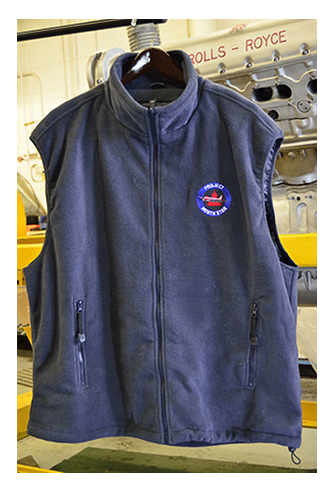
\includegraphics[scale=1.0]{fleece_YOW7578.eps}
%   %caption of the figure 
%   \caption*{\small \em PNSAC winter apparel}
%   %label of the figure, which has to correspond to \ref{}:
%   \label{fig:merchandise}
%\end{figure}




\begin{footnotesize}
    \raggedleft PNSAC\\
\end{footnotesize}

%\begin{multicols}{2}

% End of text.

%%% Local Variables: 
%%% mode: latex
%%% TeX-master: main_document.tex
%%% End: 
 
% \end{article}

%\pagebreak


% Forthcoming events ................................................. %

%\begin{article}
%   
% Template PNSAC newsletter - Miscellany
% Language: Latex
\vspace{25mm}

\title{Calendar of Events}

\maketitle

\end{multicols}

\begin{tabbing}
%June 5, 2014     \hspace{50mm}\= Board of Directors' Meeting\\
%{\normalfont\color{red}May 02, 2015}   \hspace{50mm}\= 
%{\normalfont\color{red}Members' Quarterly Meeting}\\
\textbf{Saturday, January 19, 2019}   \hspace{48mm}\=  Members Meeting \& 70th
anniversary events\\
%  Add blank line
 \> \\
\textbf{Saturday, April 13, 2019}   \hspace{52mm}\=  Annual General Meeting\\ 
 \> \\
\textbf{Sunday, June 1, 2, 2019}   \hspace{54mm}\=  Doors Open Ottawa
(Tentative Event)\\ 
 \> \\
\textbf{Monday, July 1, 2019}   \hspace{58mm}\=  Canada Day\\ 
%\textbf{Saturday, May 6, 2017}   \hspace{50mm}\=  \\ 
\end{tabbing}
%\vspace{-5mm}

\begin{multicols}{2}

%%% Local Variables: 
%%% mode: latex
%%% TeX-master: main_document.tex
%%% End: 

 
%\end{article}
%
%\pagebreak


% Board members/contact info ......................................... %

\begin{article}
  
% Template PNSAC newsletter - Contact information
% Language: Latex


\title{Board Members' Contact Information}

\maketitle

\section{PNSAC Executive}
%\label{sec:misc_pnsac_executive}

%\begin{minipage}{\columnwidth}

\address{Richard Lodge\\
Director, President\\
\email{president@projectnorthstar.ca}}

%\address{Bill Tate\\
%Director, Vice President; Special Events, Quarterly Meetings \\
%613-523-8817\\
%\email{billtate@bell.net}}

\address{Bruce Gemmill\\
Director, Project Manager; Membership\\
\email{membership@projectnorthstar.ca}}


\address{Garry Dupont\\
Director, Project Manager}\\


%\end{minipage}

%\columnbreak

%\begin{minipage}{\columnwidth}

%\address{Bruce Grant\\
%Director, NStar Chronicle Editor\\
%\email{editor@projectnorthstar.ca}}


  
%\address{Drew Hodge\\
%Director, ewsletter typesetting, website, social media\\
%\email{ldhodge@gmail.com}}
  
\address{Phil Chrysler\\
Director, Merchandise}\\

\columnbreak  

\address{Roger Button\\
Director, Corporate Secretary, NStar Chronicle Editor}\\

\address{Paul Labranche\\
Treasurer\\
\email{treasurer@projectnorthstar.ca}}

%\end{minipage}
  
\subsection{Newsletter\protect\footnote{This newsletter is typeset using
    \LaTeX.  The style package used for the newsletter (PNSAC.sty) is
    a modification of GRASSnews.sty belonging to the Geographic
    Analysis Resources Support System (GRASS). The modification was
    made possible by kind permission of the Editor-in-Chief of
    GRASS-News.}}


\small\address{Editor: Roger Button\\
\small\email{editor@projectnorthstar.ca}}

\address{Typesetter: Drew Hodge}

%\end{multicols}

%\vspace{5mm}

%\hspace{-10mm}
%\setlength\fboxrule{2pt}%
%\framebox{%
%\begin{minipage}{1\columnwidth}%
%\begin{center}
%If you would like to contribute an article to the NStar Chronicle,
%please contact Bruce Grant at 
%\par\end{center}

%\begin{center}
%\email{r_b_grant@yahoo.ca} 
%\par\end{center}

%\begin{center}
%Your comments on the contents of this issue are also appreciated.
%\par\end{center}%
%\end{minipage}}

%\begin{multicols}{2}

%\address{PNSAC Newsletter postal and Web site addresses:}


\scriptsize\address{PNSAC\\
P.O.Box 44005\\
Ottawa, ON\\
K1K 4P8}\\

\scriptsize\address{Web site: {\normalfont\color{blue}\texttt{\url{http://www.projectnorthstar.ca}}}\\
	General enquiries:\email{info@projectnorthstar.ca}}



\begin{figure}
    \centering
    \mbox{\subfigure{ \href{http://www.facebook.com/PNSAC/}{
\includegraphics[scale=0.1]{../images/facebook_128x128.pdf}}}\quad
    \subfigure{ \href{http://twitter.com/PnsacComms/}{
\includegraphics[scale=0.1]{../images/twitter_128x128.pdf}}}}
\end{figure}









%\begin{footnotesize}
%This newsletter is typeset using \LaTeX
%  \end{footnotesize}

%%% Local Variables: 
%%% mode: latex
%%% TeX-master: main_document.tex
%%% End: 
 
\end{article}


%\textit{All photos by Guy Poirier.}

\end{document}

% \begin{figure}[htbp]
%    \vspace{2em}
%    \centering
%    %name of the graphic, without the path AND in EPS format:
%    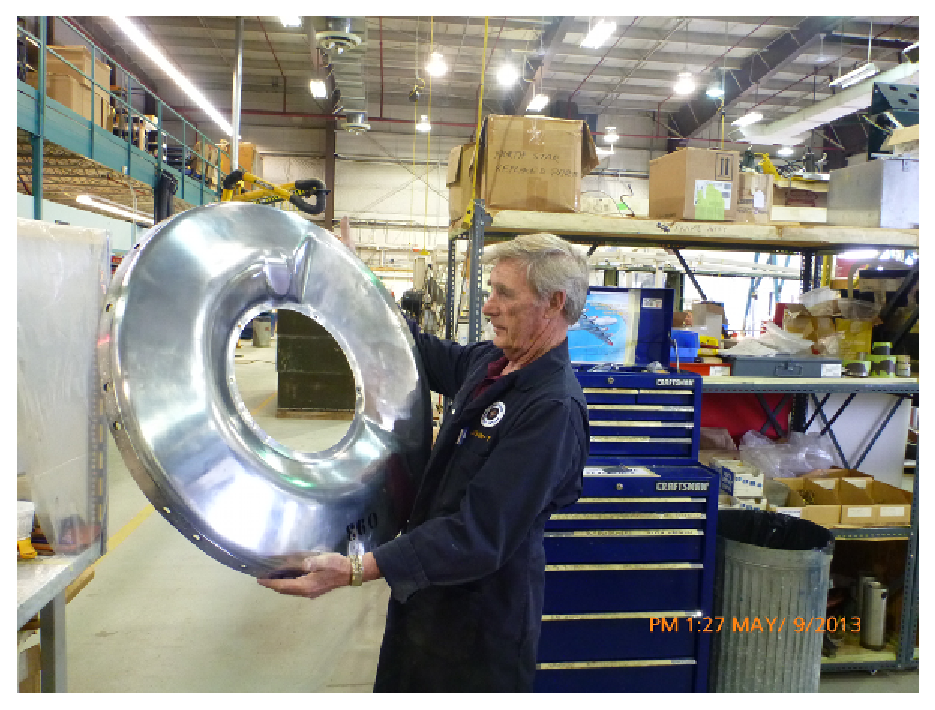
\includegraphics[scale=0.5]{engine3_prop_cowl.eps}
%    %caption of the figure 
%    \caption*{\small \em John Thibert with the propeller cowl for
%      engine nr 3.}
%    %label of the figure, which has to correspond to \ref{}:
%    \label{fig:engine3propcowl}
% \end{figure}

%%% Local Variables: 
%%% mode: latex
%%% TeX-master: main_document.tex
%%% End: 
